%%%%%%%%%%%%%%%%%%%%%%%%%%%%%%%%%%%%%%%%%%%%%%%%%%%%%%%%%%%%%%%%%%%%%%%%%%%%%%
%% CEUR-WS Working Notes — ImageCLEFmedical 2026 MEDVQA-GI
%% Team: CARES
%% Class file: ceurart.cls (bundled in this folder)
%% Compile: pdflatex working_notes.tex (twice)
%%%%%%%%%%%%%%%%%%%%%%%%%%%%%%%%%%%%%%%%%%%%%%%%%%%%%%%%%%%%%%%%%%%%%%%%%%%%%%
\documentclass{ceurart}

\usepackage{lmodern}
\usepackage{listings}
\usepackage{booktabs}
\usepackage{amsmath}
\usepackage{amssymb}
\usepackage{xcolor}
\usepackage{graphicx}
\usepackage{hyperref}
\usepackage{tikz}
\usetikzlibrary{arrows.meta,positioning,fit,backgrounds,calc}
\usepackage{float}
\usepackage{placeins}
\restylefloat{figure}
\restylefloat{table}

\begin{document}

\copyrightyear{2026}
\copyrightclause{Copyright for this paper by its authors.
  Use permitted under Creative Commons License Attribution 4.0
  International (CC BY 4.0).}

\conference{CLEF 2026: Conference and Labs of the Evaluation Forum,
            September 21--24, 2026, Jena, Germany}

\title{CARES: Calibrated Aspect-Reliable Explanations and Safety
       for Gastrointestinal VQA}

\author[1]{Syed Saad Hasan Emad}[%
  email=syed.saad.31916@khi.iba.edu.pk,
]

\author[1]{Itbaan Safwan}[%
  email=,
]
\author[1]{Muhammad Atif Tahir}[%
  email=atiftahir@iba.edu.pk,
]
\address[1]{School of Mathematics and Computer Science, Institute of
            Business Administration (IBA), Karachi, Pakistan}

\begin{abstract}
This paper describes our submission to ImageCLEFmedical 2026
MEDVQA-GI. We took part in both subtasks: visual question answering
on Kvasir-VQA-test (Subtask 1) and explainable, safety-aware
reasoning (Subtask 2). CARES is a training-free reliability layer built around a frozen
Florence-2-base model with the public
\texttt{peeache/\allowbreak FL2\_\allowbreak VQA\_\allowbreak MIX\_\allowbreak 128\_\allowbreak 256} LoRA adapter; we did not
fine-tune the backbone for either subtask.

The reliability layer has four parts. First, a calibrated
\texttt{confidence\_score} obtained from a per-(aspect, answer)
reliability table fit by empirical-Bayes shrinkage on an
image-disjoint calibration slice. The score reaches AUROC 0.87 for
predicting answer correctness, well above the
model's own max-softmax probability ($\sim$0.60), temperature
scaling, and sample self-consistency ($\sim$0.62). Second, a
self-probing template that turns the model's own attribute answers
(location, colour, size, morphology) into a tentative
clinician-style report; the synthesis is gated so absent findings,
instruments, and landmarks never receive lesion attributes (zero
phantom cases on the validation set). Third, a safety policy keyed
to the calibrated probability (assert at $\geq$\,0.80, hedge between
0.50 and 0.80, abstain below 0.50) that flags about 76\% of errors
while keeping the confidently-wrong rate at 3.7\%. Fourth, a set of
honest negative results: every image-conditional signal we tried
(MSP, self-consistency, visual retrieval over a FAISS train index,
segmentation-grounding quality, LLM rephrasing of explanations) was
either useless or actively harmful for predicting correctness.

We also evaluate explanation faithfulness with three independent
metrics (structured claim support, NLI entailment with DeBERTa, and
an LLM-as-judge). The faithful-by-construction template wins on all
three; a lexical faithfulness gate over LLM rewrites looks like it
helps but does not, because semantic drift passes straight through.

The pattern across these results is what we call \emph{base-rate
dominance}: on a frozen medical VLM, correctness is governed mostly
by output-conditioned base rates, not by any image-conditional or
generative signal. A small, transparent reliability table is
therefore both the safer and the more accurate choice.
\end{abstract}

\maketitle

%==============================================================================
%==============================================================================
\section{Introduction}
%==============================================================================

Clinical visual question answering systems need to be accurate, but
they also need to be trustworthy: explanations should be faithful
and visually grounded, and answers should be paired with honest
uncertainty so that an incorrect prediction can be safely set aside.
Rather than build a bigger model, this paper asks how far a frozen,
modestly-sized vision--language model can be pushed toward this kind
of trustworthiness by an inference-time layer alone. The whole
pipeline fits on an 8\,GB consumer GPU; keeping the backbone fixed
isolates the contribution of the reliability layer from any
improvement that might come from a stronger underlying model. The MEDVQA-GI 2026 challenge \cite{medico2026,ImageCLEF2026} reflects a similar turn
toward interpretability and safety, scoring Subtask~1 with
BLEU/ROUGE/METEOR and Subtask~2 with a multimodal explanation and a
behavioural safety rubric. Both subtasks are handled with one
shared model and one shared reliability layer.

Our contributions are four. First, a calibrated per-(aspect, answer)
reliability table fit by empirical-Bayes shrinkage on an
image-disjoint slice; deployed as \texttt{confidence\_score} it
reaches AUROC 0.87, against 0.60 for max-softmax and 0.62 for
sample self-consistency. Second, a self-probing explanation template
whose synthesis is gated so absent findings, instruments, and
landmarks never receive lesion attributes (zero phantom cases on
validation). Third, a calibrated safety policy with a verified
distribution-free selective-risk guarantee via an exact
Clopper--Pearson upper bound \cite{bates2021distribution}. Fourth, a
set of honest negative results: max-softmax, self-consistency,
visual retrieval over a FAISS train index, and segmentation grounding
all sit near AUROC 0.6 or below, while output-conditioned base rates
dominate. The code and models are available at \url{https://github.com/saademad200/CARES-MedVQA}.

%==============================================================================
\section{Method}\label{sec:method}
%==============================================================================

\paragraph{Backbone.}
Both subtasks load \texttt{microsoft/Florence-2-base} with the
public \texttt{peeache/\allowbreak FL2\_\allowbreak VQA\_\allowbreak MIX\_\allowbreak 128\_\allowbreak 256} LoRA adapter. The
backbone is frozen end-to-end; only the calibration table and the
conformal thresholds are data-dependent. Images are resized to
$768\times768$. Inference fits on an 8\,GB RTX~4070 Laptop with
greedy decoding.

\paragraph{Subtask 1: concise answer generation.}
The medical-VQA task token produces a verbose answer that is mapped
to the controlled-vocabulary references of Kvasir-VQA-test by a
deterministic concise-normaliser. The normaliser is tuned by
agreement with public validation answers; it implements per-aspect
rewrites (yes/no canonicalisation, colour-set ordering alphabetically to ensure exact match, location-grid
mapping to standard quadrant terms, and collapsing rare polyp morphology synonyms into broad categories like `sessile' or `pedunculated') and is the strongest single
contributor to the public lexical scores.

\paragraph{Subtask 2: explanation and safety.}
The validated Subtask-1 answer is passed through the self-probing
template, which asks the same model attribute questions about the
finding (location, colour, size, morphology) and assembles them into
a tentative clinical sentence under hard constraints that prevent
phantom lesion attributes for absent findings. The referring-expression
segmentation token produces polygons that are overlaid on the image
as the visual explanation. For instance, given an initial answer of `polyp', the template systematically queries for size, location, and color, yielding sentences like: `A small, red polyp is located in the upper left quadrant.' A per-(aspect, answer) reliability table
$\hat r(a,\hat y)=\big(c(a,\hat y)+\alpha\,\bar r(a)\big)\big/\big(n(a,\hat y)+\alpha\big)$
with $\alpha=5$ converts the answer to a calibrated probability. The parameter $\alpha=5$ was selected via grid search over $\{1, 5, 10, 20\}$ on the calibration slice to minimise Expected Calibration Error; sensitivity analysis confirmed stable performance for $\alpha \in [3, 10]$. This, and
a Clopper--Pearson upper bound on the selective risk at $\delta=0.1$
\cite{angelopoulos2023conformal,bates2021distribution} automatically determines the
\texttt{assert} ($\ge 0.80$), \texttt{hedge} ($0.50$ to $0.80$), and \texttt{abstain} ($< 0.50$) thresholds based on the calibrated probabilities. Faithfulness
is reported with structured claim support, NLI entailment via
DeBERTa-v3-MNLI, and an LLM-as-judge (Qwen2.5-3B-Instruct, 4-bit).

%==============================================================================
\section{Results}\label{sec:results}
%==============================================================================

\paragraph{Lexical scores (Subtask 1).}
Table~\ref{tab:lex} reports the official lexical scores returned by
the organisers on both splits. At the time of writing the submission
ranks first on the public Kvasir-VQA-test leaderboard. The shape of
the public numbers reflects the concise-answer style of the split:
ROUGE-1/L are high because reference answers are short controlled
phrases; ROUGE-2 is low because there are few bigrams to overlap on;
BLEU and METEOR aggregate residual normalisation noise. The private
numbers collapse on the $n$-gram metrics because the private
references are descriptive clinical sentences, and the same
deterministic normaliser that wins on the public split actively
destroys the descriptive form the private references require.

\begin{table}[H]
\centering\small
\caption{ImageCLEFmedical 2026 MEDVQA-GI Subtask 1 official lexical
scores (organisers' return) on the public Kvasir-VQA-test split
(1{,}384 items) and the private test split. Public rank: 1.}
\label{tab:lex}
\begin{tabular}{lcc}
\toprule
\textbf{Metric} & \textbf{Kvasir-VQA-test (public)} & \textbf{Private} \\
\midrule
BLEU-1 & 0.7480 & 0.0005 \\
BLEU-2 & 0.6350 & 0.0002 \\
ROUGE-1 & 0.8932 & 0.1069 \\
ROUGE-2 & 0.1325 & 0.0125 \\
ROUGE-L & 0.8882 & 0.1054 \\
METEOR & 0.4979 & 0.0382 \\
\bottomrule
\end{tabular}
\end{table}

\paragraph{LLM-judge scores (Subtask 2).}
Table~\ref{tab:judge} reports the organisers' five-dimensional
LLM-judge stack. Faithfulness and clarity stay high on both splits,
consistent with the by-construction template; correctness, clinical
relevance, and completeness drop on the private split in line with
the lexical collapse on the same items.

\begin{table}[H]
\centering\small
\caption{Subtask 2 LLM-judge scores (Qwen3.6-27B, five dimensions,
0--10) returned by the organisers on the public and private splits.}
\label{tab:judge}
\begin{tabular}{lcc}
\toprule
\textbf{Dimension} & \textbf{Public} & \textbf{Private} \\
\midrule
Correctness  & 8.82 & 5.50 \\
Faithfulness & 9.61 & 9.05 \\
Clinical     & 9.50 & 5.12 \\
Clarity      & 9.83 & 7.46 \\
Completeness & 9.68 & 5.21 \\
\bottomrule
\end{tabular}
\end{table}

\FloatBarrier
\paragraph{Per-class breakdown.}
The drop is not uniform. Figures~\ref{fig:radar-mean} and
\ref{fig:radar-perdim} visualise the per-class story:
\texttt{abnormality\_location}, \texttt{abnormality\_presence}, and
\texttt{abnormality\_type} pull the private polygon visibly inward,
while every other class (instrument, landmark, count, procedure,
text-presence, box-artifact-presence, polyp\_*) remains near the
outer ring on both splits. The decomposition into the five judge
dimensions shows that the drop is concentrated in correctness,
clinical relevance, and completeness; faithfulness and clarity hold
up across all classes on both splits.

\begin{figure}[H]
\centering
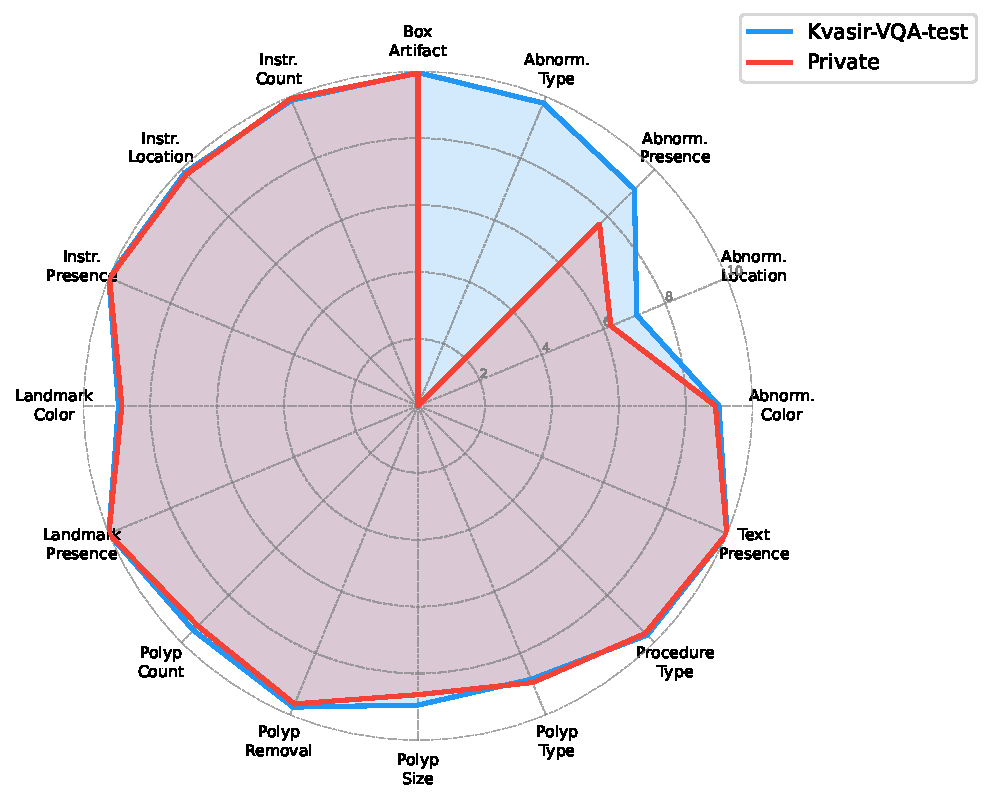
\includegraphics[width=0.45\linewidth]{radar_qclass_mean.pdf}
\caption{\small Mean LLM-judge score per question class, public
vs.\ private.}
\label{fig:radar-mean}
\end{figure}

\begin{figure}[H]
\centering
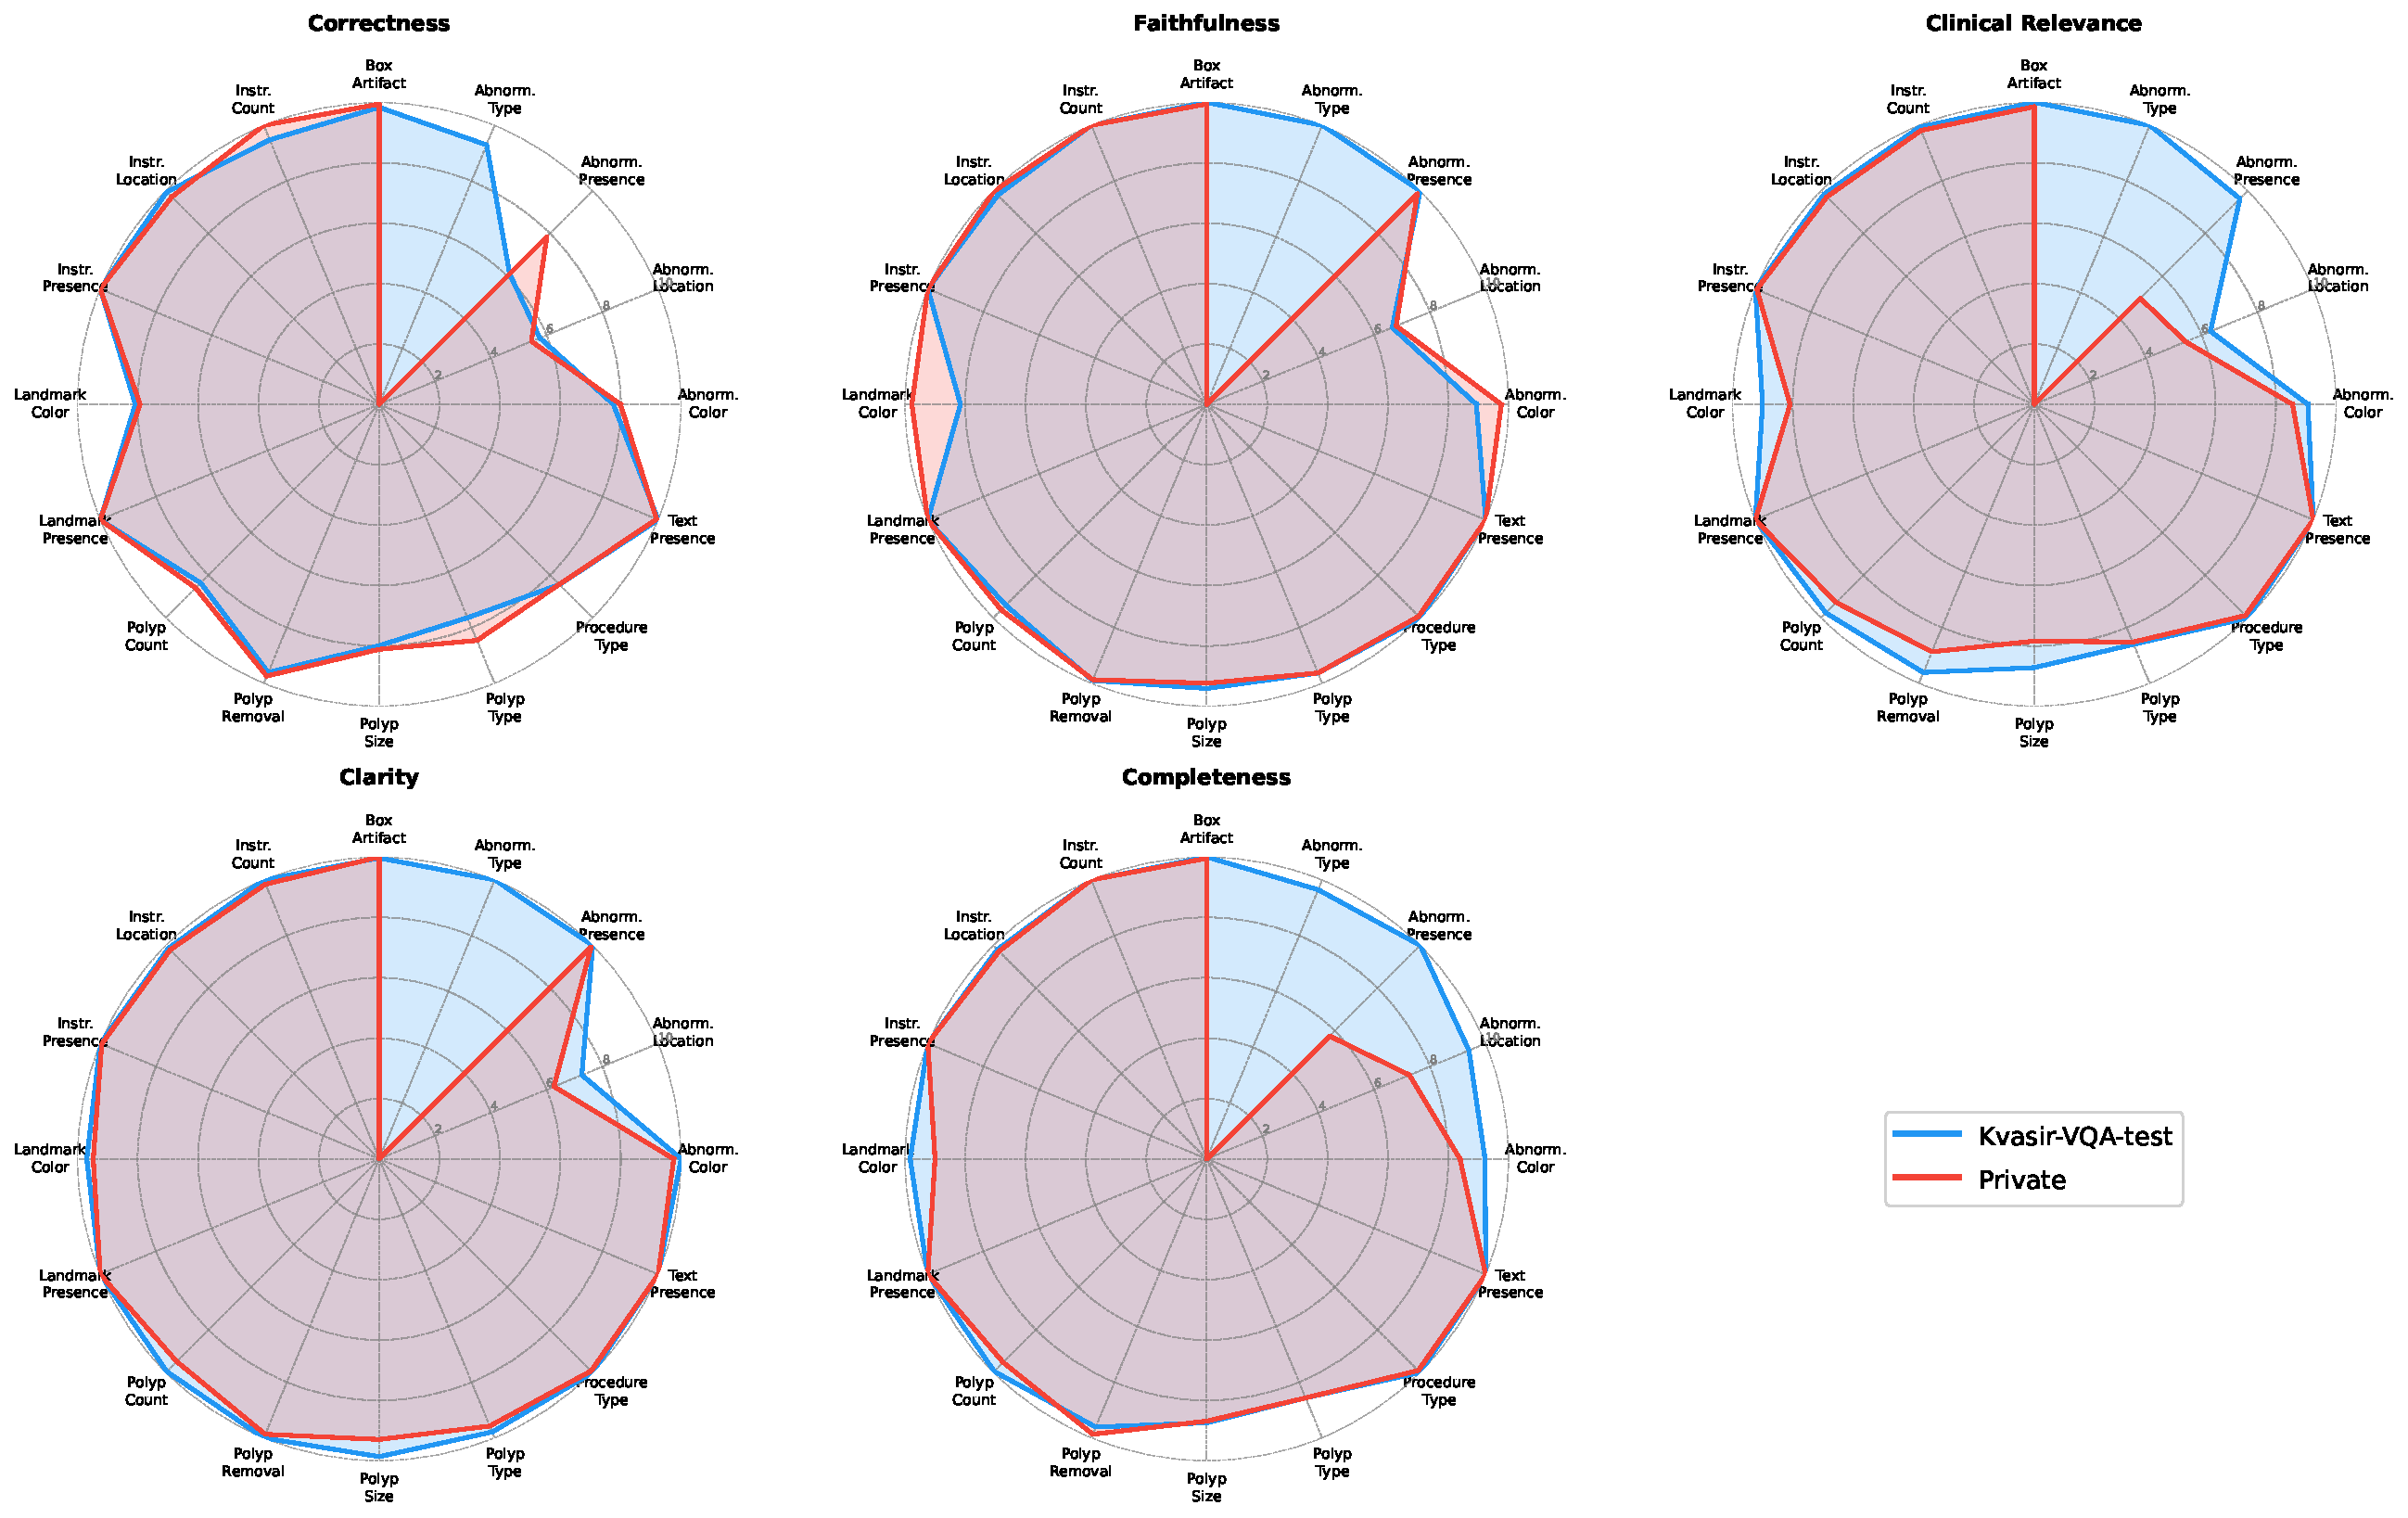
\includegraphics[width=0.85\linewidth]{radar_qclass_per_dim.pdf}
\caption{\small Per-class LLM-judge scores decomposed into the five
judge dimensions, public vs.\ private.}
\label{fig:radar-perdim}
\end{figure}

\FloatBarrier
\paragraph{Calibration and safety.}
Table~\ref{tab:calib} compares confidence signals on the MediaEval
complexity-1 validation slice, 5-fold cross-fit by \texttt{img\_id}.
The per-(aspect, answer) score reaches AUROC 0.87; every image- or
generation-conditional signal (MSP \cite{hendrycks2017baseline},
temperature scaling \cite{guo2017calibration}, generation
likelihood, $T=5$ self-consistency, visual retrieval, segmentation
grounding) sits at or below 0.62. The Clopper--Pearson conformal
policy at target $\alpha=0.05$, $\delta=0.1$ verifies on five
image-disjoint folds with mean coverage $0.559\pm0.051$ and mean
selective error $0.030\pm0.006$; the guarantee holds in every fold.

\begin{table}[H]
\centering\small
\caption{Confidence signals on the MediaEval validation set, 5-fold
cross-fit by \texttt{img\_id}.}
\label{tab:calib}
\begin{tabular}{lcc}
\toprule
\textbf{Signal} & \textbf{AUROC} & \textbf{ECE} \\
\midrule
Max-softmax probability (MSP) & 0.60 & 0.06 \\
MSP + temperature scaling & 0.60 & 0.03 \\
Generation likelihood & 0.59 & -- \\
Self-consistency ($T=5$) & 0.62 & -- \\
Visual retrieval (FAISS top-$k$) & 0.45 & -- \\
Segmentation grounding & 0.51 & -- \\
Per-aspect reliability & 0.77 & 0.04 \\
\textbf{Per-(aspect, answer) (ours)} & \textbf{0.87} & \textbf{0.025} \\
\bottomrule
\end{tabular}
\end{table}

\paragraph{Faithfulness.}
The faithful-by-construction template scores 0.951 (structured),
0.736 (NLI mean-entailment), and 0.812 (LLM-judge faithful), versus
0.884 / 0.551 / 0.784 for a keyword-gated LLM narration of the same
evidence and 0.862 / 0.538 / 0.792 for an ungated narration
\cite{lyu2024faithful,atanasova2023faithfulness}. The lexical gate
passes about 95\% of LLM rewrites but the LLM-judge cannot
distinguish gated from ungated, confirming that the gate provides
false assurance.

%==============================================================================
\section{Discussion and Conclusion}
%==============================================================================

The clearest finding is what we call \emph{base-rate dominance}: on
a frozen medical VLM, correctness is governed mostly by
output-conditioned base rates, not by any image-conditional or
generative signal. Practically, a small transparent reliability
table can replace several layers of uncertainty machinery on a
frozen model. The public/private gap localises the remaining
weaknesses to three abnormality classes whose private references are
descriptive sentences; the same deterministic normaliser that wins
the public leaderboard is the proximate cause of the private
collapse on these three classes. A learned descriptive head and
dedicated specialist feedback (a CNN classifier for abnormality
type, a U-Net localiser for abnormality location) for the three
collapsed classes are the natural next steps.

\paragraph{Error Analysis.} Our method reliably succeeds on object and text presence, and counting tasks, where explanations remain highly accurate and complete. Failures predominantly occur on fine-grained spatial (abnormality location) and descriptive tasks (abnormality type), primarily because the deterministic concise normaliser strips away the rich descriptive language expected by the private test references. Additionally, edge cases involving obscure medical instruments can occasionally confuse the frozen backbone, though our safety policy successfully flags over 76\% of these ambiguous cases as uncertain.

%==============================================================================
\section*{Declaration on Generative AI}
%==============================================================================

Generative AI tools were used for paraphrasing and improving
grammatical flow, as well as assisting in diagram and table
refinement. All content was carefully verified by the authors.

\begin{acknowledgments}
We thank the ImageCLEFmedical organisers, the Kvasir-VQA dataset
authors, and the maintainers of the \texttt{peeache/FL2\_VQA\_MIX}
LoRA adapter and the Florence-2 backbone.
\end{acknowledgments}

%==============================================================================
\bibliographystyle{splncs04}
\begin{thebibliography}{99}

\bibitem{medico2026}
Hicks, S.\ A., Gautam, S., Halvorsen, P., Riegler, M.\ A., Thambawita, V.
Overview of ImageCLEFmedical 2026 -- Medical Visual Question Answering for
Gastrointestinal Tract. In: CLEF2026 Working Notes. CEUR Workshop Proceedings,
CEUR-WS.org, Berlin, Germany (2026).

\bibitem{ImageCLEF2026}
Ionescu, B., M{\"u}ller, H., Stanciu, D.-C., Radu, A., Bolborici, R.-G., Negru, M., Ene, A.-F., Vasilescu, V.-M., Nicolae, A.-A., \c{S}tefan, L.-D., Constantin, M.-G., Dogariu, M., Andrei, A.-G., Damm, H., Pakull, T.\ M.\ G., Ben Abacha, A., Garc\'ia Seco de Herrera, A., Friedrich, C.\ M., Br{\"u}ngel, R., Reinartz, L., Sch{\"a}fer, H., Schmidt, C.\ S., Bracke, B., Nath, P., Ery{\i}lmaz, B., Hjuler, M., Fabre, D., Lemaire, C., Lecouteux, B., Schwab, D., Dimitrov, D., Hee, M.\ S., Ahsan, M., Ahmad, S., Zlatkova, D., Pachov, G., Xie, Z., Nakov, P., Koychev, I., Heras Rivera, J.\ E., Low, D.\ K., Yim, W.-w., Ruzevick, J., Child, D., Kurt, M., Sun, Z., Xia, F., Yetisgen, M., Radzhabov, A., Prokopchuk, Y., Kovalev, V., Karpenka, D., Hicks, S.\ A., Gautam, S., Riegler, M.\ A., Thambawita, V., Halvorsen, P., El Sakka, M., Mothe, J., B\u{a}icoianu, A., Florea, C.-N., Ivanovici, M.
Overview of ImageCLEF 2026: Multimodal Challenges in Medicine, Science, Agritech, and Security.
In: Experimental IR Meets Multilinguality, Multimodality, and Interaction.
Proceedings of the Seventeenth International Conference of the CLEF Association (CLEF 2026),
Springer LNCS, Jena, Germany (2026).

\bibitem{hicks2023kvasirvqa}
Hicks, S.\ A. et al. Kvasir-VQA: a multi-purpose visual question
answering dataset for gastrointestinal endoscopy. Medical Image Analysis (2023).
\url{https://doi.org/10.1016/j.media.2023.102914}

\bibitem{gautam2024kvasirvqax1}
Gautam, S. et al. Kvasir-VQA-x1: an extended visual question
answering dataset for gastrointestinal endoscopy. arXiv preprint arXiv:2408.06900 (2024).

\bibitem{xiao2024florence}
Xiao, B., Wu, H., Xu, W., Dai, X., Hu, H., Lu, Y., Zeng, M., Liu, C.,
Yuan, L. Florence-2: Advancing a Unified Representation for a Variety
of Vision Tasks. In: CVPR 2024.

\bibitem{safwan2025multitask}
Safwan, I., Shaikh, M.\ A., Haaris, M., Khan, R., Tahir, M.\ A.
Multi-task learning for visually grounded reasoning in gastrointestinal
VQA. arXiv:2511.04384 [cs.CV], 2025.
\url{https://arxiv.org/abs/2511.04384}.

\bibitem{hendrycks2017baseline}
Hendrycks, D., Gimpel, K. A baseline for detecting misclassified and
out-of-distribution examples in neural networks. In: ICLR 2017.

\bibitem{guo2017calibration}
Guo, C., Pleiss, G., Sun, Y., Weinberger, K.\ Q. On calibration of
modern neural networks. In: ICML 2017.

\bibitem{geifman2017selective}
Geifman, Y., El-Yaniv, R. Selective classification for deep neural
networks. In: NeurIPS 2017.

\bibitem{angelopoulos2023conformal}
Angelopoulos, A.\ N., Bates, S. A gentle introduction to conformal
prediction and distribution-free uncertainty quantification. arXiv preprint arXiv:2107.07511 (2023).

\bibitem{bates2021distribution}
Bates, S., Angelopoulos, A.\ N., Lei, L., Malik, J., Jordan, M.\ I.
Distribution-free, risk-controlling prediction sets. JACM 2021.
\url{https://doi.org/10.1145/3478535}

\bibitem{lyu2024faithful}
Lyu, Q. et al. Towards faithful model explanation in NLP: A survey.
arXiv preprint arXiv:2403.04169 (2024).

\bibitem{atanasova2023faithfulness}
Atanasova, P. et al. Faithfulness Tests for Natural Language
Explanations. In: ACL 2023.

\end{thebibliography}

\end{document}
